% !Mode:: "TeX:UTF-8"

\chapter{算法轻量化设计与实现}

\section{引言}
对于实际的红外无人机目标检测任务,任务环境常常是野外开阔地带,因此
检测算法常常需要在移动设备上运行,而对于移动端嵌入式设备,硬件的运算能力和成本都十分有限,因此对算法的内存占用和运行时间有更高的要求。也就是在保证检测精度的同时也要保证实时性,这就需要对算法进行一定程度的轻量化,降低算法的内存占用和运行时间,使得移动端设备也可以实时实现红外无人机目标检测。
本章将在上文提到的算法基础上,应用Ghost模块对算法模型进行轻量化,并且在PC端和移动端NVIDIA AGX XAVIER设备上进行算法的性能测试,并对实验结果进行分析。

\section{神经网络模型轻量化}
随着现在的各种计算机视觉任务的发展,为了实现更加复杂的功能,相应的神经网络模型的层数越来越深,参数量也越来越大。实验数据表明,训练一个具备更多参数的大型网络往往能使得算法取得更好的性能,因为大型网络往往可以在原本的高精确度表现下降不多的同时适当地减少冗余参数,相比一开始就训练一个较小的网络,训练大型网络再进行轻量化往往能在目标检测精度和参数量上取得更好的平衡。

\subsection{模型剪枝}
因为卷积神经网络往往用于复杂的图像处理任务,因此网络模型的结构一般都比较复杂,模型网络深度较大,随之带来模型占用内存空间过大和计算量过大的问题,于是一些研究者就想从对网络模型剪枝的方式直观地压缩模型的整体体积。
Hassibi等人\cite{hassibi1992second}在研究了利用训练数据和网络结构信息求逆Hessian矩阵H-1的递推关系来进行网络权重修减的方法并通过实验测试后,基于此方法得到了一种称为“最优脑科医生”(Optimal Brain Surgeon)的模型剪枝方法,这种方法能够在网络权重数量较小的情况下仍然保持很好的泛化能力。
Yihui He等人\cite{he2017channel}针对深度较大的卷积神经网络进行了模型权重修建的研究,提出了一种创新的剪枝方法。该剪枝方法针对给定模型的每一层进行处理,具体地,将每一次迭代分成选择通道和最小二乘法重建两个步骤,并将这个微观过程应用到整个网络模型中。该算法的主要优势在于对不同网络结构都有较好的适用性,在ResNet等网络中进行实验后证明该剪枝算法能取得较好的性能。

Sajid Anwar等人\cite{anwar2017structured}研究分析了很多网络剪枝中存在的难点,例如剪枝会导致网络模型的结构一定程度上受到破坏,使得原本的模型出现不规则的连接结构。盲目的对网络进行剪枝常常会使得模型的并行加速算法不再适用,从而拖慢算法的推理速度。针对上述问题Sajid Anwar等人提出了一种结构化的剪枝方法,核心思想是对各个权重分析其重要性,保留分类计算中真正起到关键作用的网络部分,同时对重要性较低的部分进行修剪。实验证明该结构化剪枝方法能在精度损失很小的前提下大幅减少
模型的参数量。

\subsection{参数量化}
除了上文提到的对网络模型中的某些权重参数做直接删减操作外,还可以通过对模型的某些参数进行占用空间的压缩,即参数量化的方法,对模型的内存占用进行优化。简单地说量化过程就是将参数的数据类型进行压缩,比如从占用32bit空间的浮点型参数变为占用16bit空间的整型参数。毫无疑问量化后每个参数可以表达的权重范围和精细度都会降低。

\subsection{知识蒸馏}
高性能的深度学习网络通常是计算型和参数密集型的,难以应用于资源受限的边缘设备  为了能够在低
资源设备上运行深度学习模型,需要研发高效的小规模网络。  知识蒸馏是获取高效小规模网络的一种新兴方法,
其主要思想是将学习能力强的复杂教师模型中的“知识”迁移到简单的学生模型中。  同时,它通过神经网络的互
学习、自学习等优化策略和无标签、跨模态等数据资源对模型的性能增强也具有显著的效果。  基于在模型压缩和
模型增强上的优越特性,知识蒸馏已成为深度学习领域的一个研究热点和重点。 

\subsection{改进网络结构}
除了通用的剪枝、量化、知识蒸馏等模型轻量化方法之外,常用的使神经网络更高效的方法是设计新型网络。
常见的轻量网络模型有SqueezeNet、Xception、MobileNet、ShuffleNet等。每种网络都提出了一种或几种特殊结构用来减少模型的参数量或者提升模型的推理速度。

(1)SqueezeNet
SqueezeNet\cite{iandola2016squeezenet}的主要策略是用$1\times1$的卷积代替部分$3\times3$的卷积运算,这使得卷积的参数数量减少了9倍。此外,SqueezeNet还减少了$3\times3$卷积的通道数。一个$3\times3$卷积的计算量是$3\times3 \times M \times N$(其中$M$和$N$分别是输入通道数和输出通道数),作者将$M$和$N$减少来达到减少整个模型的参数量的目的。另外,为了提升网络的精度,SqueezeNet将下采样模块后置。作者认为较大的Feature Map含有更多的信息,因此将下采样往分类层移动。这样的调整会提高模型的精度,同时也会增加计算量。
同时,SqueezeNet的缺点也很明显,SqueezeNet意图面向的场景是移动端实时运行,但是该算法实际的处理策略是用更大的深度来换取网络整体参数量的减少,但是这样改进之后网络的并行加速优化空间十分有限,算法的推理时间往往更大,并没有达到更好地服务移动端计算设备的目的。

(2)Xception
深度可分离卷积率先是由 Laurent Sifre在其博士论文中提出。这篇文章主要从Inception\cite{szegedy2015going}的角度出发,探讨了Inception和深度可分离卷积的关系,从一个全新的角度解释了深度可分离卷积。再结合stoa的残差网络\cite{he2016deep},作者提出了一种新型的轻量网络结构Xception。Xception取义自Extreme Inception,表示Xception是一种极端的Inception。
Inception模块对实现卷积运算的处理方法是,通过对各种尺寸卷积核的组合并添加池化等模块,使得模型在占用更少空间的前提下捕捉到更丰富的特征。该算法的核心思想是将卷积操作分成获取空间相关性信息和获取通道相关性信息两个独立的步骤。

(2)MobileNet
MobileNet\cite{howard2017mobilenets}模型是Google针对手机等嵌入式设备提出的一种轻量级的深层神经网络,该网络的核心处理模块便是深度可分离卷积。
MobileNet模型基于深度可分离卷积搭建,这是分解卷积的一种形式,它将标准卷积分解为深度卷积和以$1\times1$卷积构成的逐点卷积。对MobileNet而言,深度卷积针对每个输入通道应用一个卷积核。然后逐点卷积应用$1\times1$卷积来聚合输出。标准卷积将过滤核聚合输入形成一系列输出融合成一步。深度可分离卷积分解成两层,一层用于过滤,一层用于聚合。

% 设标准卷积层的输入维度为$D_{F} \times D_{F} \times M$,输出特征图维度为$D_{F} \times D_{F} \times N$,

% 其中$D_{F}$表示一个正方形输入特征图的宽和高,$M$表示输入通道数,$D_{G}$指的是正方形输出特征图的宽和高,$N$表示输出通道数。设标准卷积核大小为$D_{K} \times D_{K} \times M \times N$,其中$D_{F}$是卷积核的空间维度,$M$表示输入通道数,$N$表示输出通道数,则标准卷积的计算消耗为
% \begin{equation}
%     D_{K} \times D_{K} \times M \times N \times D_{F} \times D_{F}
% \end{equation}

% 其中计算成本乘法取决于输入通道的数量$M$、输出通道的数量$N$、内核大小$D_{K} \times D_{K}$和特征图大小$D_{F} \times D_{F}$。MobileNet模型使用深度可分离卷积来打破输出通道数量和内核大小之间的相互作用。
% 标准的卷积运算具有填充效果,基于卷积核的特征和组合特征以产生新的表征。过滤和组合步骤可以通过使用称为深度可分离卷积的分解卷积为2个步骤,以显著降低计算成本。

% 深度可分离卷积由两部分组成:深度卷积和逐点卷积。我们使用深度卷积来针对每个通道使用一个卷积核。逐点卷积通过使用$1\times1$卷积来针对深度卷积的输出实现线性变换。MobileNet在两个层中都使用了BN和ReLU。深度卷积的计算成本为:
% \begin{equation}
%     D_{K} \times D_{K} \times M \times D_{F} \times D_{F}
% \end{equation}

% 相对于标准卷积,深度卷积是非常有效的。但是它只过滤输入通道,不聚合它们形成新的特征。所以提供针对深度卷积的输出实现线性变换的额外层,即$1\times1$卷积层用于生成新特征。

% 深度卷积和$1\times1$卷积(逐点卷积)的联合称为深度可分离卷积。
% 深度可分离卷积的计算成本为:
% \begin{equation}
%     D_{K} \times D_{K} \times M \times D_{F} \times D_{F}+M \times N \times D_{F} \times D_{F}
% \end{equation}

% 是深度卷积和逐点卷积的操作和。

% 通过将卷积表示为过滤和组合两步过程,可以得到计算量的减少比例:
% \begin{equation}
%     \frac{D_{K} \times D_{K} \times M \times D_{F} \times D_{F}+M \times N \times D_{F} \times D_{F}}{D_{K} \times D_{K} \times M \times N \times D_{F} \times D_{F}}=\frac{1}{N}+\frac{1}{D_{K}^{2}}
% \end{equation}

% MobileNet通过使用$3\times3$的深度可分离卷积,相对于标准卷积而言计算量减少了8-9倍。

\section{基于Ghost卷积的网络结构轻量化}
Ghost 模块是一种替代传统CNN中的卷积操作并且获得更快速度和更小模型体积的思想\cite{han2020ghostnet}。通过对比分析ResNet-50网络第一个残差组(Residual group)输出的特征图可视化结果,发现一些特征图高度相似。如果按照传统的思考方式,可能认为这些相似的特征图存在冗余,是多余信息,想办法避免产生这些高度相似的特征图。而Ghost模块另辟蹊径,选择以一种更简单的操作来生成相同数量的特征图,从而实现更快速高效的检测。本文进行了Ghost模块的具体实现,并将其与YOLOv5网络相结合,以达到算法轻量化的目的。

\subsection{Ghost模块思想}
典型的卷积计算过程如图\ref{conv}所示,所有的输入逐一经过卷积运算后生成新的特征图。这里的每一个输出张量都是一个由卷积核运算产生的特征图。但是这些特征图中可能有些特征图相似度较高,因此可以认为两张或几张比较相似的特征图是产生于几次同样代价的卷积是一种浪费。

\begin{figure}[htbp]
    \centering
    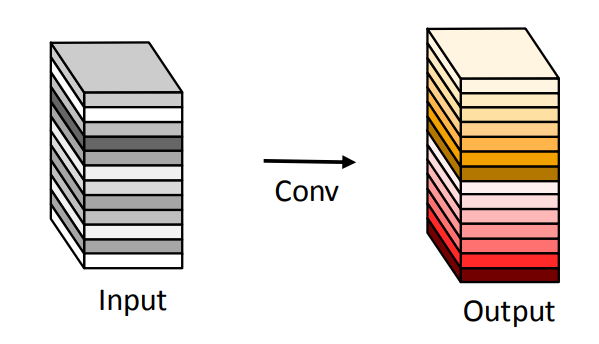
\includegraphics[width = 0.5\textwidth]{传统卷积.png}
    \caption{传统卷积示意图}
    \label{conv}
\end{figure}

如图\ref{identical}所示,每次卷积的所有输出中,可以找到一些相互之间相似度较高的特征图。设图中的A, A’、B B’相似度较高,可以设计一种计算方法替代生成A’和B’的卷积运算,从而达到减小计算量的目的。

\begin{figure}[htbp]
    \centering
    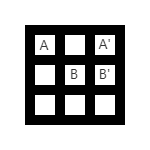
\includegraphics[width = 0.5\textwidth]{重复特征图.png}
    \caption{重复特征图示意图}
    \label{identical}
\end{figure}

\begin{figure}[htbp]
    \centering
    \includegraphics[width = 0.9\textwidth]{Ghost卷积.png}
    \caption{Ghost卷积示意图}
    \label{Ghost1}
\end{figure}

如图\ref{Ghost1}所示,Ghost模块的做法是用一些更小的卷积核(即参数更少运算更快)替代原先的卷积部分,但是这部分卷积核产生的输出量只能达到相当于本来卷积输出量的一部分,这时根据上文对相似特征图的分析,可以采用一些线性变换的方式去生成剩下的特征图,从而达到用更轻量的卷积滤波器去生成相同规模特征图的目的。

\subsection{基于Ghost模块的模型轻量化算法实现}

\begin{figure}[htbp]
    \centering
    \includegraphics[width = 0.6\textwidth]{Ghost算法实现.png}
    \caption{Ghost算法实现示意图}
    \label{Ghost2}
\end{figure}

本课题的Ghost实现流程如图\ref{Ghost2}所示,将原始卷积层改变成两部分,分别产生相当于原始卷积层一半通道数的输出(实际上二者的输出比例可以任意调节),可以使得改进后的模块参数量减少。

具体地,本文在实现Ghost模块时采用的简单线性变换是分组卷积。图\ref{convp}表示了普通卷积模块的卷积过程,而图\ref{Ghostp}表示本文实现的Ghost模块的卷积过程。从图\ref{convp}中可以看出,普通卷积的一个卷积核对应一个输出通道,每个卷积核和所有输入通道进行运算;而在图\ref{Ghostp}中,首先对输入通道$C_1$应用普通卷积,产生$\frac{C_2}{2}$个输出特征图,此后应用分组个数为$\frac{C_2}{2}$的分组卷积,每个分组内的卷积核不与组外的输入特征图进行运算,分组卷积再产生$\frac{C_2}{2}$个输出特征图,因此可以实现Ghost模块的输出特征图和普通卷积的输出特征图维度相同。
\begin{figure}[htbp]
    \centering
    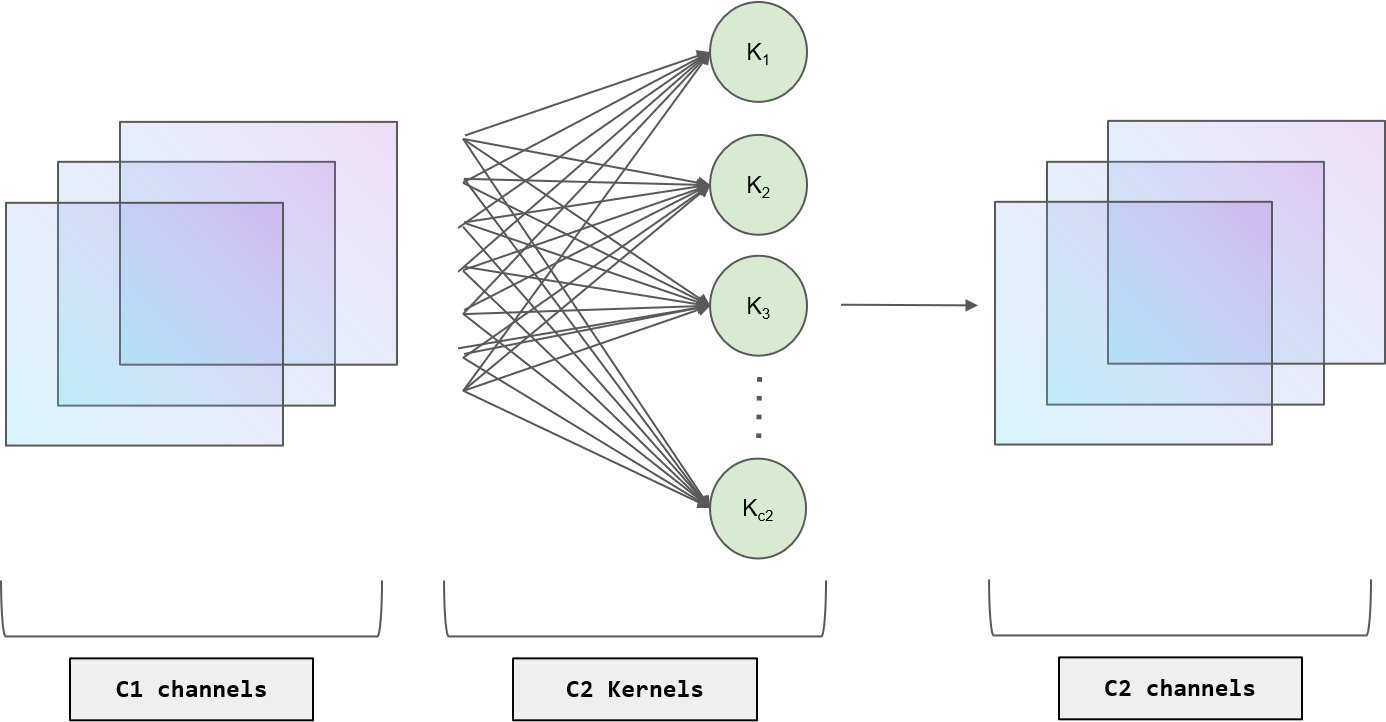
\includegraphics[width = 0.8\textwidth]{普通卷积过程.png}
    \caption{普通卷积实现示意图}
    \label{convp}
\end{figure}

\begin{figure}[htbp]
    \centering
    \includegraphics[width = 0.8\textwidth]{Ghost卷积过程.png}
    \caption{Ghost卷积实现示意图}
    \label{Ghostp}
\end{figure}

\begin{figure}[htbp]
	\centering
	\begin{minipage}{0.49\linewidth}
		\centering
		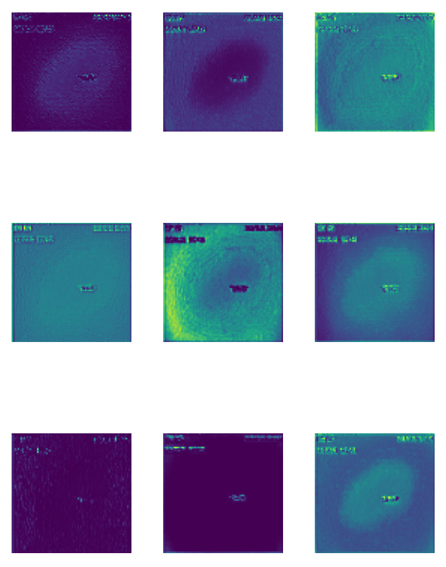
\includegraphics[width=0.9\linewidth]{convfmap.PNG}
		\caption{普通卷积特征图}
		\label{convf}%文中引用该图片代号
	\end{minipage}
	%\qquad
	\begin{minipage}{0.49\linewidth}
		\centering
		\includegraphics[width=0.9\linewidth]{Ghostfmap.PNG}
		\caption{Ghost卷积特征图}
		\label{Ghostf}%文中引用该图片代号
	\end{minipage}
\end{figure}

普通卷积和Ghost卷积产生的特征图如图\ref{convf}和图\ref{Ghostf}所示,从图中可以看出,由于Ghost卷积相当于对普通卷积进行了一定程度的转化,所以Ghost卷积产生的特征图和普通卷积产生的特征图存在一定的差别,不过图\ref{convf}和图\ref{Ghostf}中确实有相当大比例的对应位置特征图是相似的,这也验证了上文的理论分析。此外,由于Ghost卷积减少了网络结构中的参数,所以在简化运算、加速推理的同时,各特征图之间的差异更小,也就是Ghost卷积产生的特征图在一定程度上丢失了多样性,也将导致整个网络失去一些特征,降低最终目标检测的精度。

\subsection{Ghost算法理论分析}
对于特定的网络结构,在将传统卷积模块替换成Ghost卷积模块之后,可以对网络模型的参数数量和推理速度进行理论计算,得出改进后网络相对于原网络的推理加速比和参数压缩比。

(1)相对于普通卷积模块的加速比

\begin{equation}
    \begin{aligned}
    r_{s} &=\frac{n \times h^{\prime} \times w^{\prime} \times c \times k \times k}{\frac{n}{s} \times h^{\prime} \times w^{\prime} \times c \times k \times k+(s-1) \times \frac{n}{s} \times h^{\prime} \times w^{\prime} \times d \times d} \\
    &=\frac{c \times k \times k}{\frac{1}{s} \times c \times k \times k+\frac{s-1}{s} \times d \times d} \approx \frac{s \times c}{s+c-1} \approx S
    \end{aligned}
    \label{jsb}
\end{equation}

如式\ref{jsb}所示,设输入通道数为$c$,输出通道数为$n$,输入图像高度为$h^{\prime}$和$w^{\prime}$,其中保留的原始卷积通道数为本来的$1/s$,原始卷积核大小为$k*k$,线性核大小为$d*d$,由于线性变换是在每个通道上进行,所以代表线性变换的一项中不含输入通道数$c$。

由式\ref{jsb}可得,将原始卷积模块替换为一半卷积一半线性变换的Ghost模块后(即将$s=2$代入),可以得到该模块的理论提速比为2。

(1)相对于普通卷积模块的参数压缩比

\begin{equation}
    r_{c}=\frac{n \times c \times k \times k}{\frac{n}{s} \times c \times k \times k+(s-1) \times \frac{n}{s} \times d \times d} \approx \frac{s \times c}{s+c-1} \approx \frac{s c}{c}=S
    \label{csys}
\end{equation}

如式\ref{csys}所示,经过计算可以得到改进后的Ghost模块和改进之前的普通卷积模块理论参数压缩比为2。

\subsection{Ghost算法实验对比分析}
将Ghost模块对应改动部署到YOLOv5网络之后,在实验平台上进行测试验证。分别用YOLOv5网络模型和调整深度之后得到的小型网络(记为YOLOv5s)作为参照,验证YOLOv5+Ghost在红外无人机图像数据集上的效果。
本章提到的算法用Pytorch框架进行网络部署和测试。操作系统为Windows 10,算法实现依赖的软件环境为python。实验采用的服务器CPU型号为Intel Core i7-11700k,GPU型号为NVIDIA GeForce RTX 3080Ti,GPU搭载的显存容量为12GB。

\begin{table}[htbp]
    \caption{不同算法对红外无人机数据集的检测结果}
    \vspace{0.5em}\centering\wuhao
    \begin{tabular}{ccccc}
    \toprule
    检测算法 & mAP & 推理时间(ms) & 参数量 & 计算量(GFLOPs)\\
    \midrule
    YOLOv5 & 0.937 & 2.5 & 7.0M & 15.8\\
    YOLOv5s & 0.901 & 1.5 & 3.6M & 8.6\\
    Ours(YOLOv5+Ghost)& 0.915 & 1.2 & 3.7M & 8.1\\
    \bottomrule
    \end{tabular}
    \label{t22}
\end{table}

从表\ref{t22}中可以看出,减少卷积核数量的YOLOv5s相比于YOLOv5网络,已经在参数量和计算量上大大减少,同时推理时间也在缩短,这是因为YOLOv5s网络是对YOLOv5网络进行卷积核尺寸、个数的缩减后得出的,因而YOLOv5s网络的特征提取能力更弱,在红外无人机数据集上的检测精度也更低。而本文提出的YOLOv5+Ghost算法相比YOLOv5s算法能获得更高的检测精度和更快的推理速度,在参数量和计算量上和YOLOv5s算法持平。

\section{轻量化红外无人机目标检测算法嵌入式实现与验证}
为了进一步验证本文提出的轻量化红外无人机目标检测算法的有效性,本节将本文提出的完整算法模型进行转换,并且在嵌入式设备上进行检测和验证。

\subsection{嵌入式设备介绍}

本文采用的嵌入式设备是
NVIDIA
Jetson AGX Xavier。该平台是NVIDIA公司生产的新一代嵌入式人工智能计算平台,能够在各种移动系统上进行部署,大幅提高整体系统的计算处理能力。
该平台的具体参数规格如表\ref{t1}中所
示。
该移动端平台的主要特点可以概括为算力强、体积小、接口全。更多功能的接口使得NVIDIA Jetson AGX Xavier能够和各种前端设备快速协同,更加方便目标检测等图像处理算法的灵活部署。
NVIDIA Jetson AGX Xavier 嵌入式开发平台如图
\ref{agx}所示。

\begin{figure}[htbp]
    \centering
    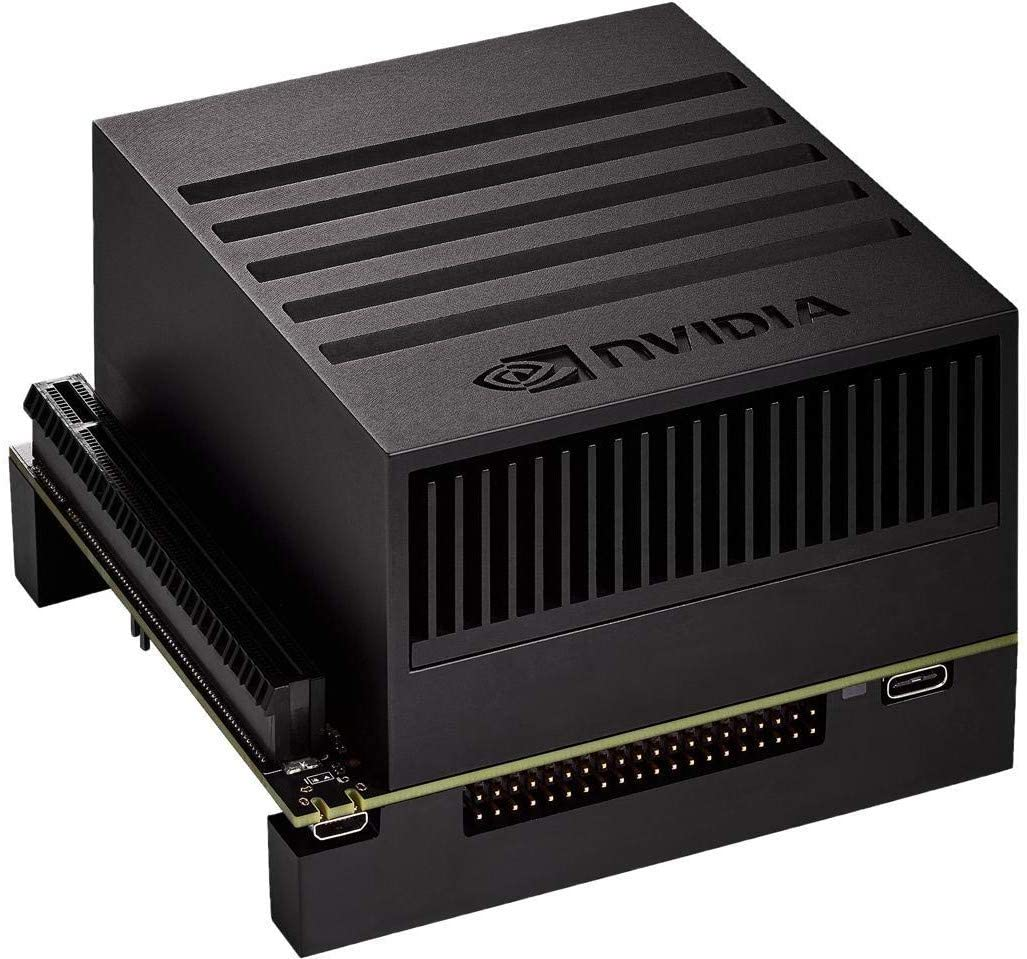
\includegraphics[width = 0.5\textwidth]{agx.jpg}
    \caption{NVIDIA Jetson AGX Xavier实物图}
    \label{agx}
\end{figure}

\begin{table}[htbp]
    \caption{NVIDIA Jetson AGX Xavier参数规格}
    \vspace{0.5em}\centering\wuhao
    \begin{tabular}{cc}
    \toprule
    项目 & 规格\\
    \midrule
    GPU & 512核 NVIDIA Volta GPU,64 Tensor核\\
    CPU & 8核 ARM v8.2 64-bit CPU, 8MB L2 + 4MB L3\\
    DL Accelerator & 2x NVDLA\\
    Vision Accelerator & 2x PVA\\
    Memory & 32GB 256-bit LPDDR4x\\
    Storage & 32GB eMMC 5.1\\
    CSI Camera & 16 lanes MIPI CSI-2\\
    PCIe & x16 connector with x8 PCIe Gen4 or x8 SLVS-EC\\
    Networking & RJ45 (Gigabit Ethernet)\\
    尺寸 & 105mm x 105mm x 65mm\\
    \bottomrule
    \end{tabular}
    \label{t1}
\end{table}

\subsection{ONNX框架}
现如今,各大主流深度学习框架都有着自己独有的特点与魅力,吸引着广大科研与开发人员,例如:
(1)Caffe2:方便机器学习算法和模型大规模部署在移动设备。

(2)PyTorch:PyTorch是一个快速便于实验深度学习框架。但是由于其高度封装,导致部分function不够灵活。

(3)TensorFlow:TensorFlow 是一个开放源代码软件库,是很多主流框架的基础或者依赖。几乎能满足所有机器学习开发的功能,但是也有由于其功能代码过于底层,学习成本高,代码冗繁,编程逻辑与常规不同等缺点。

此外还有:Cognitive Toolkit (CNTK),Apache MXNet,Chainer,Apple CoreML,SciKit-Learn,ML.NET

深度学习算法大多通过计算数据流图来完成神经网络的深度学习过程。 一些框架(例如CNTK,Caffe2,Theano和TensorFlow)使用静态图形,而其他框架(例如PyTorch和Chainer)使用动态图形。 但是这些框架都提供了接口,使开发人员可以轻松构建计算图和运行时,以优化的方式处理图。 这些图用作中间表示(IR),捕获开发人员源代码的特定意图,有助于优化和转换在特定设备(CPU,GPU,FPGA等)上运行。

对于本课题的红外无人机目标检测的任务场景,模型的移动设备部署需要借助tensorrt模型来进行实现,这时候如果把整个模型再重新采用tensorrt进行搭建和训练,无疑是消耗大量的时间和精力。这时就可以用ONNX这样的中间框架来进行已训练模型的转换。

开放式神经网络交换(ONNX)是迈向开放式生态系统的第一步,它使AI开发人员能够随着项目的发展选择合适的工具。 ONNX为AI模型提供开源格式。 它定义了可扩展的计算图模型,以及内置运算符和标准数据类型的定义。 最初的ONNX专注于推理(评估)所需的功能。 ONNX解释计算图的可移植,它使用graph的序列化格式。 它不一定是框架选择在内部使用和操作计算的形式。 例如,如果在优化过程中操作更有效,则实现可以在存储器中以不同方式表示模型。

\subsection{TensorRT框架}
TensorRT 是 NVIDIA 研制的AI推理框架,可以让深度学习模型在GPU上实现更加高性能的部署和推理。TensorRT 支持 Caffe,TensorFlow,Mxnet,Pytorch 等深度学习框架。TensorRT 是一个 C++ 库,并且提供了 C++ API 和 Python API,主要在 NVIDIA GPU 进行高性能的推理 (Inference) 加速。

\subsection{嵌入式平台算法实现及分析}
借助ONNX框架和TensorRT框架,本文实现了轻量化红外无人机目标检测的engine格式模型,以使得第3章和第4章前半部分中研究的基于深度学习的轻量化红外图像无人机目标检测算法进行转换后的算法模型在 NVIDIA AGX XAVIER平台上可以进行推理测试。

\begin{figure}[htbp]
    \centering
    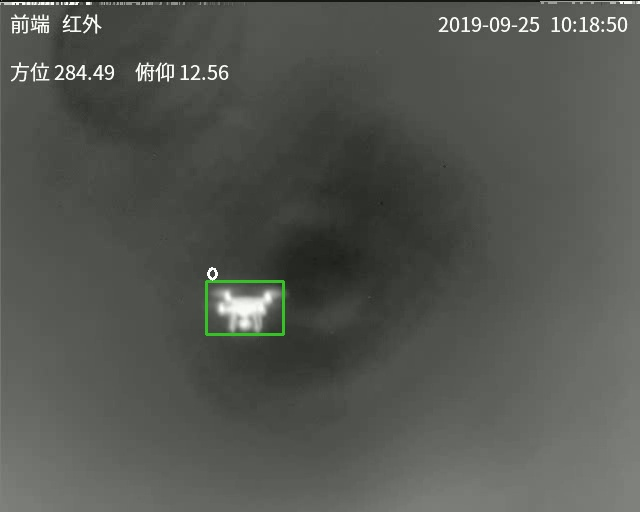
\includegraphics[width = 0.5\textwidth]{agx结果.jpg}
    \caption{嵌入式设备检测结果图}
    \label{agxo}
\end{figure}

算法在嵌入式平台上的检测效果如图\ref{agxo}所示。经过测试,本文提出的算法经过轻量化后在NVIDIA AGX XAVIER平台上的mAP为0.90,推理时间为36ms,运行速度为28FPS,在保证精度较高的前提下,基本满足实时检测的要求。

\section{本章小结}
本章目的在于将无人机目标检测算法移植到嵌入式平台NVIDIA AGX XAVIER上实现实时检
测。首先介绍了深度学习网络模型轻量化的常用方法,并且选择了一种目标检测领域性能较好的方法即Ghost模块替代法。然后用Ghost卷积对第3章的算法模型进行压缩,通过在PC平台和在嵌入式平台NVIDIA AGX XAVIER上的测试,证明了本文提出的算法能在红外无人机目标数据集上取得较高的检测精度,并且该算法的轻量化版本能在嵌入式平台上在占用较小内存空间的同时基本实现实时检测。

